\documentclass{article}
\usepackage{polyglossia}

\usepackage{hyperref}
\hypersetup{
    pdfencoding=auto,
    pdftitle={Data Compression in High Energy Physics; Master's Thesis Projects},
    pdfauthor={Roel Aaij},
    pdfcreator={LaTeX},
    pdfproducer={LuaTex 1.0.4},
    colorlinks,
    linkcolor=,
    urlcolor=links
}
\usepackage[export]{adjustbox}
\usepackage{graphicx}
\usepackage{amsmath}
\usepackage{amsthm}
\usepackage{wasysym}
\usepackage{pict2e}
\usepackage{ifthen}

\usepackage{fontspec}
\usepackage{unicode-math}
\setsansfont[Ligatures=TeX]{Linux Biolinum O}
\setmathfont{Latin Modern Math}
\setmathfont[range=\mathit/{latin,Latin,num,Greek,greek}]{Linux Biolinum O Italic}
\setmathfont[range=\mathup/{latin,Latin,num,Greek,greek}]{Linux Biolinum O}
\setmathfont[range=\mathbfup/{latin,Latin,num,Greek,greek}]{Linux Biolinum O Bold}
\setmathfont[range={"221E}]{Linux Biolinum O}% "0221E = \infty

\usepackage{caption}
\captionsetup{labelformat=empty,labelsep=none}

\title{Challenge for GSoC 2019 Project on Speeding up KM3NeT's Reconstruction}
\author{Roel Aaij}

\begin{document}

\section{Description of KM3NeT}

\begin{figure}
  \center
  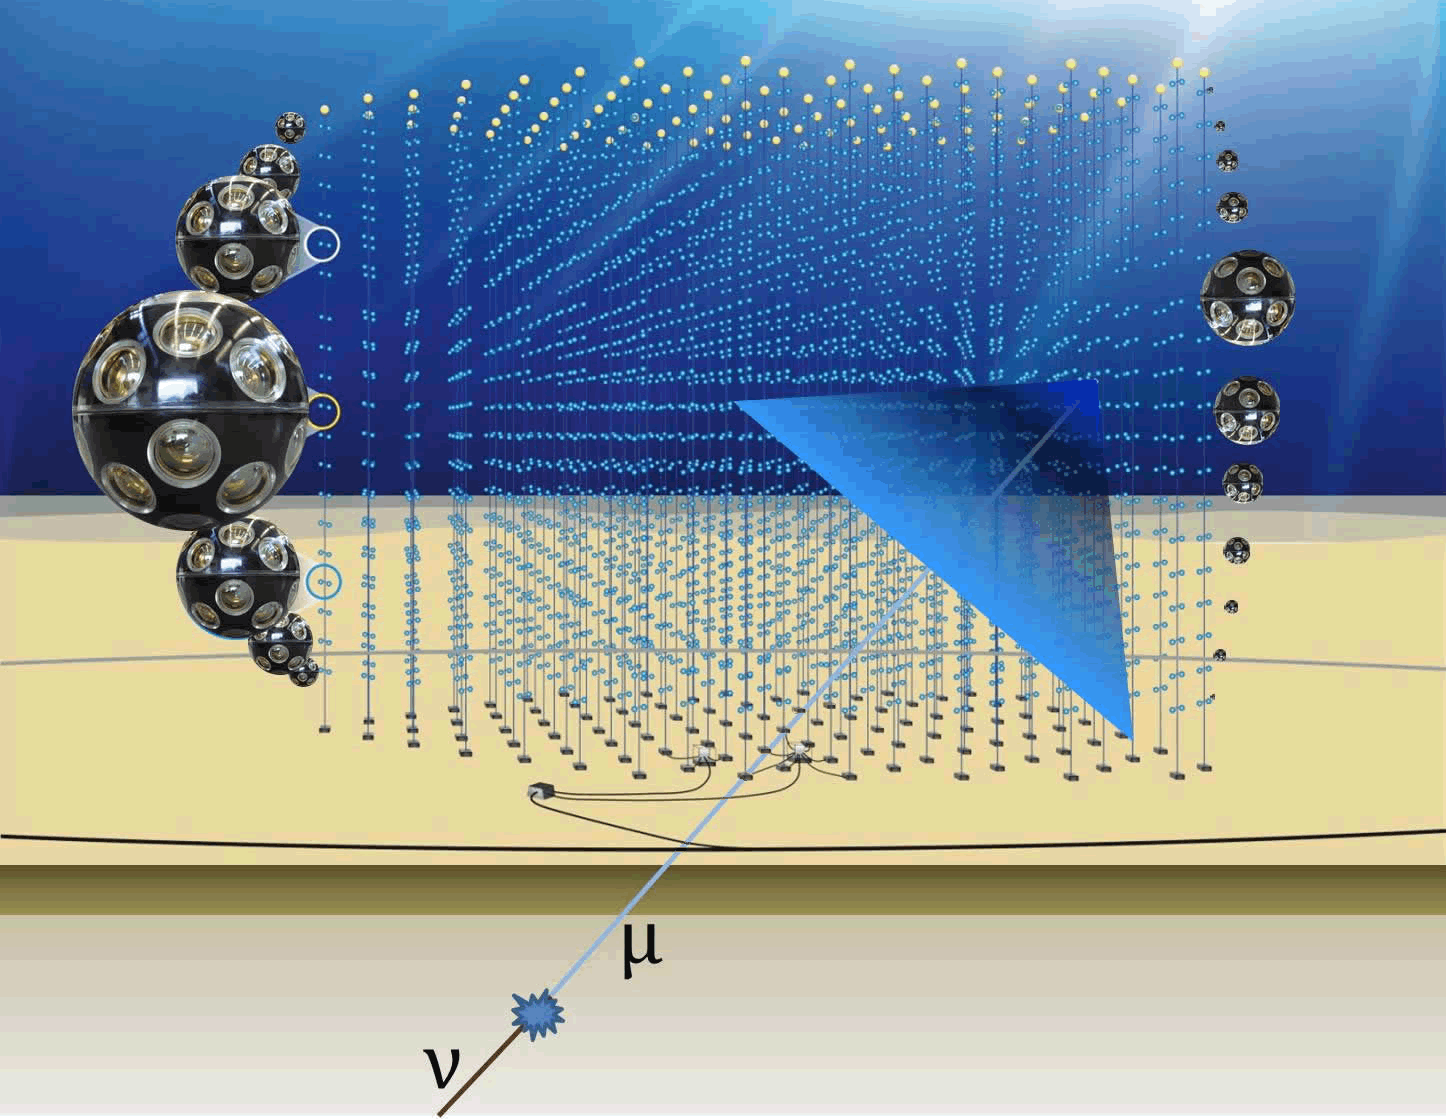
\includegraphics[width=0.8\textwidth]{KM3NeT-NeutrinoToMuon.png}
  \caption{A muon traversing the KM3NeT detector}
\end{figure}

KM3NeT is an underwater research facility that houses two large
neutrino telescopes: ORCA and ARCA. The ORCA telescope consists of a
number of strings of optical modules attached to the floor of the
Mediterranean Sea off the coast of Toulon in France.

The optical modules each contain 31 photomultiplier tubes (PMTs) that
detect light emitted by muons and electrons that traverse water inside
the detector. Some of these muons and electrons are created by
interactions of neutrinos with the water or sea floor. These are the
muons and electrons that KM3NeT aims to detect and whose trajectory
and energy it aims to reconstruct.

\section{Background Generator Library}

There are also several other sources of light present in the water,
which result in so-called background noise. A standalone generator
that simulates such noise is available at
\href{https://github.com/nlesc-km3net/k40gen}{https://github.com/nlesc-km3net/k40gen}

\section{Challenge}

The code for this challenge is available on the GSoC_2019 branch of
the k40gen repository. It consists of a skeleton file located in the
``challenge'' subdirectory.



\end{document}
